\chapter{Composing a solver}
\label{chapter:composingats}
\smtrat contributes a toolbox for composing an SMT compliant solver for its supported logics, that means it is incremental, supports backtracking and provides reasons for inconsistency. The resulting
solver is either a fully operative SMT solver, which can be applied
directly on \texttt{.smt2}-files, or a theory solver, which can be embedded into an SMT 
solver in order to extend its supported logics by those provided by \smtrat.

We are talking about composition and toolbox, as \smtrat contains implementations
of many different procedures to tackle, \eg \supportedLogics, each of them
embedded in a module with uniform interfaces. These modules form the tools in the toolbox
and it is dedicated to a user how to use them for solving an SMT formula.
We provide a self-explanatory graphical user interface (GUI) for the definition of a graph-based 
strategy specifying which module(s) should be applied on which formula, 
taking into account the modules which were already involved.

In Section~\ref{sec::strategy} we have already introduced
a strategy and in the following of this chapter we firstly give a brief introduction 
to the existing modules equipped with an estimation of their input-based performances and then illustrate
how to use the GUI for composing a strategy.

\section{Existing module implementation}
\subsection{The \cnferModuleClass}
Transforms its received formula into conjunctive normal form CNF.

\paragraph{Efficiency} The worst case complexity of this module is polynomial in the number of operators in the formula to transform.

\subsection{The \satModuleClass}
This module abstracts it's received formula, being any SMT formula of the supported logics of \smtrat, to it's Boolean skeleton. It thereby replaces all constraints in the formula by fresh Boolean variables. The resulting propositional formula is then solved with \minisat~\cite{minisat}, where after each completed decision level the constraints belonging to the assigned Boolean variables are checked for consistency by the backends of this module. In the case of inconsistency, the infeasible subsets of the backends are abstracted and then involved in the search for a satisfying solution.

\paragraph{Efficiency} Even though the worst case complexity of this procedure, not considering the complexity of the backend calls, is exponential in the number of variables in the abstracted formula, the procedure is in practice more efficient than any of the theory modules. Hence, it does clearly not form a bottleneck of the SMT solving. However, one should aim at reducing the number and complexity of the theory (backend) calls of this module, which might be influenced by infeasible subsets, which are small and/or involve constraints of earlier decision levels in the SAT solving, and lemmas, which either prune the search space of the SAT solving or ease subsequent theory calls.

\subsection{The \lraModuleClass}
Implements the SMT compliant \emph{Simplex} method presented in \cite{DM06}.
Hence, this module can decide the consistency of any conjunction
consisting only of linear real arithmetic constraints. Furthermore,
it might also find the consistency of a conjunction of constraints
even if they are not all linear and calls a backend after removing
some redundant linear constraints, if the linear constraints are satisfiable
and the found solution does not satisfy the non-linear constraints. Note that the 
\lraModuleClass might need to communicate a lemma/tautology to a preceding 
\satModuleClass, if it receives a constraint with the relation symbol $\neq$
 and the strategy needs for this reason to define a \satModuleClass at any 
 position before an \lraModuleClass.

\paragraph{Integer arithmetic} In order to find integer solutions, this
module applies, depending on which settings are used, branch-and-bound,
the construction of Gomory cuts and the generation of cuts from 
proofs~\cite{DilligDA11}. It is also supported to combine these approaches. Note that
for all of them the \lraModuleClass needs to communicate a lemma/tautology to a
preceding \satModuleClass and the strategy needs for this reason to define a 
\satModuleClass at any position before an \lraModuleClass.

\paragraph{Efficiency} The worst case complexity of the implemented
approach is exponential in the number of variables occurring in the
problem to solve. However, in practice, it performs much faster, and
the worst case applies only on very artificial examples. This module
outperforms any module implementing a method that is designed for 
solving formulas with non-linear constraints. If the received formula
contains integer valued variables, the aforementioned methods might not
terminate.
\subsection{The \icpModuleClass}
Implements ..

\paragraph{Efficiency} ..
\subsection{The \gbModuleClass}
Implements the Gr\"obner bases based procedure as presented in~\cite{JLCA_CAI13}. In general, this procedure can detect only the unsatisfiability of a conjunction of equations. This module also supports the usage of these equations to further simplify all constraints in the conjunction of constraints forming its input and passes these simplified constraints to its backends. However, it cannot be guaranteed that backends perform better on the simplified constraints than on the constraints before simplification.

\paragraph{Efficiency} The worst case complexity of the underlying procedure is exponential in the number of variables of the input constraints. In the case that the conjunction of constraints to check for satisfiability contains equations, this module can be more efficient than other modules for NRA on finding out inconsistency.
\subsection{The \vsModuleClass}
Implements the \emph{virtual substitution} method for a conjunction of constraints as described in \cite{}. This module supports incremental calls, efficient backtracking and infeasible subset generation. Note, that the infeasible subsets are often very small but not necessarily minimal. The implemented approach is not complete, as it maybe cannot decide the satisfiability of a conjunction containing a constraint, which involves a variable with degree $3$ or more. Note, that even if no constraint of such form occurs in the received formula, this module might not be able to determine the consistency of its received formula, as it could create constraints of this form in its solving process. Nevertheless, the implemented approach is efficient compared to other approaches for non-linear real arithmetic conjunctions, and therefore well-suited to be used for solving conjunctions of non-linear real arithmetic constraints before complete approaches have their try. In combination with a backend, this module tries to solve the given problem and calls the backend on problems with less variables.

\paragraph{Efficiency} The worst case complexity of this approach is exponential in the number of real arithmetic variables occurring in the conjunction to solve. It performs especially good on almost linear instances and slightly prefers problems only containing constraints with the relation symbols $\leq$, $\geq$ and $=$. It is often the case, that even if the conjunction to solve contains many not suited constraints, this module can determine the consistency on the basis of a well suited subset of the constraints in this conjunction.
\subsection{The \cadModuleClass}
This module implements an adapted version of the \emph{cylindrical algebraic decomposition} (CAD) for a conjunction of constraints as described in \cite{Article_Collins_75}.
It extends the original algorithm to be SMT compliant and implements the ideas from \cite{Article_Loup_TubeCAD}.

The CAD method consists of two basic routines: the projection (or elimination) of polynomials and the lifting (or construction) of samples.
The projection transforms a set of polynomials over a set of variables to a new set of polynomials that do not contain some of the variables.
The lifting starts with a sample point of degree $k$ and constructs a sample point of degree $k+1$ using the polynomial sets from the projection.
Both routines work in an incremental fashion: polynomials are only projected if needed and the construction is performed as a depth-first search.

\paragraph{Efficiency} 
The worst case complexity of this algorithm is doubly exponential in the number of variables, the base being the sum of the number of polynomials and the maximum degree of any polynomial.
This is due to an quadratic increase of polynomials in each projection step and a number of possible sample points that grows with the number of polynomials.

The practical performance heavily depends on the number and degree of polynomials created during the elimination.
It benefits greatly if the real roots of the polynomials are rational, as irrational root operation may take quite some time.


\section{Specifying a strategy with the GUI}

The following subsections are used to give an overview of the 
 \smtrat's GUI, which we call \smtxrat, and to introduce its functionalities.

\subsection{Concept}
\label{sec:concept_of_smt-xrat}
The underlying concept of \smtxrat is the user-guided, visual 
modeling of module compositions in form of graphs and their 
mapping onto their corresponding source code for \smtrat. A 
modeled graph expresses an intended strategy graph of the user. 
Both can easily be projected on each other, because the data 
structure of a strategy graph also describes a graph structure, 
as explained in the previous chapter. A mapping considers not 
only the modeled hierarchy of the SMT-RAT modules, but also 
their attributes. Furthermore the GUI complies the constraints 
of these attributes during the modeling process, for example 
priority values are required to be unique.

The GUI does not only support the visual creation of strategy 
graphs and their translation into source code, but also enables 
the user to integrate the translated source code into \smtrat or, 
if necessary, delete it subsequently. The conclusive work only 
involves a recompilation of \smtrat with the desired strategy 
graph instance to obtain a customized SMT solver.

\subsection{Main window structure}
\label{sec:main_window_structure_of_smt-xrat}
The main window structure of the \smtxrat application can be seen 
in Figure \ref{fig:smt-xrat_main_window}. It principally consists 
only of one large pane, which is called \emph{strategy graph pane}. 
This pane embodies the workspace of the user and visualizes the 
composition of SMT-RAT modules, which are currently modeled. Only a
comparatively small area is occupied by a compact menu bar, which 
offers for instance the exportation of a strategy graph into \smtrat.
\begin{figure}[ht]
  \begin{center}
    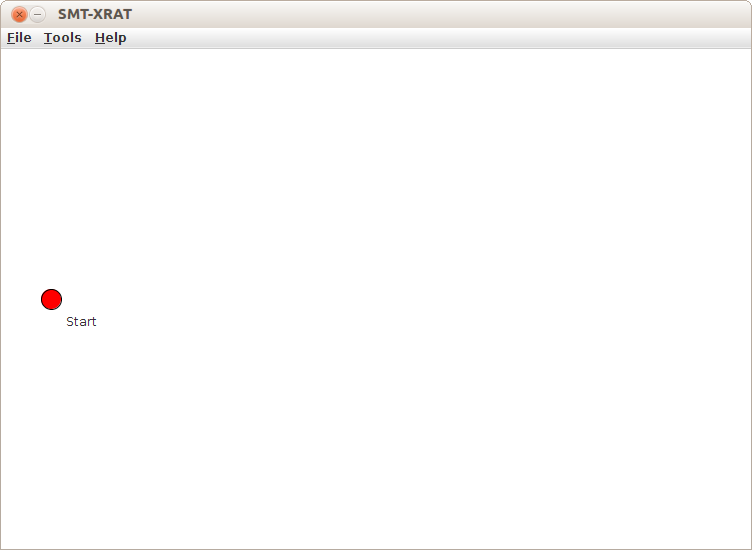
\includegraphics[width=0.9\textwidth]{graphics/smt-xrat_main_window.png}
  \end{center}
  \caption{The main window of the \smtxrat application in its initial state.}
  \label{fig:smt-xrat_main_window}
\end{figure}

\subsection{Strategy graph pane}
\label{sec:the_strategy_graph_pane}
The graphs, which can be modeled in the strategy pane, must be acyclic, directed and weakly 
connected. Nodes represent \smtrat modules and edges represent the call 
hierarchy of them. Both of the element types are labeled to display all 
necessary and editable module attributes within the visualization.
Modeling strategy graphs on the pane implies the interactive operations 
of adding, editing and deleting modules and also aligning elements, 
if desired by the user.

\subsubsection{Adding backends}
\label{sec:adding_backends}
\begin{figure}[ht]
  \begin{center}
    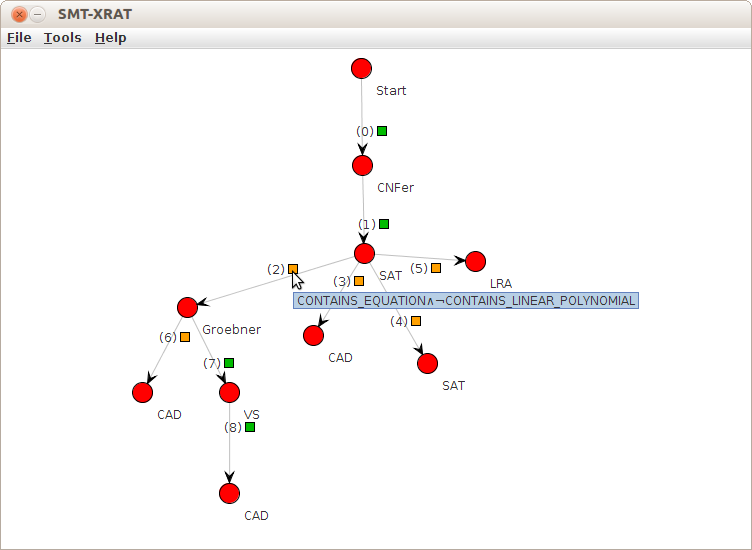
\includegraphics[width=0.9\textwidth]{graphics/smt-xrat_condition_ttt.png}
  \end{center}
  \caption{The small rectangles alongside the edges reveal the hidden condition of a backend.}
  \label{fig:smt-xrat_condition_ttt}
\end{figure}

An initial visualization of the pane contains the inevitable \emph{Start} 
module of an SMT solver, which displays no attributes, but marks the 
starting point for the user to create the desired strategy graph. 
The user can simply consider the \emph{Start} module as the front-end of an 
SMT solver where, \eg \supportedLogics formulas are passed to. Building up a composition of 
modules occurs by appending backends to the \emph{Start} module and then to 
the newly appended backends and so forth. When appending a backend to a 
selected module, a dialog window requests the operating user to input a 
condition and to choose the type of \smtrat module for the new backend. 
The GUI provides a special input interface to enter conditions, which is 
explained later. For each appended backend a new node as well as a directed 
edge from the originating module to this new node is drawn in the visualization. 
In this way, the graph gradually arises on the pane.  A node is labeled with its 
type of \smtrat module whereas an edge holds its condition and an automatically 
assigned priority value. Initially this priority value is always the total number 
of currently existing modules minus $1$, as the \emph{Start} module is not 
counted. As the user-defined conditions might get quite long, they cannot be directly 
seen on the strategy graph pane. Instead, a small rectangle alongside the 
edge reveals them quickly on request. The user needs to point the mouse cursor 
over a rectangle to obtain its corresponding tool tip text, which shows the 
hidden condition, as can be seen in Figure \ref{fig:smt-xrat_condition_ttt}.
This leaves the graph compact and helps to concentrate on the more essential 
aspect of modeling an execution hierarchy. The user can choose to input an 
own condition or leave it by the default value of `\texttt{TRUE}', which, as 
described before, means that given a formula the condition is always satisfied and,
hence, the backends will always be used. 
To point out better which modules contain default conditions and which do not,
the color of a rectangle containing a default condition is green and otherwise 
orange.

\subsubsection{Grammar for conditions}
\label{sec:grammar_for_backend_conditions}
When adding a module to the strategy graph pane, the user has to input a valid
condition for its intended use as backend. A valid condition is a derivation of 
the formal Grammar 
\[{\cal C}=(N, \Sigma, R, S).\] 
The set of nonterminals is given by 
\[N=\{S, T, B, C, D, P\},\] 
whereas the set of terminal symbols 
\[\Sigma=\{\texttt{(}, \texttt{)}, \neg, \leftrightarrow, \oplus, \rightarrow, \land, \lor\} \cup \{\texttt{TRUE}, \texttt{p}_1, \dots, \texttt{p}_n \}\]
consists of the union of logical operators and propositions. $S \in N$ is the 
start symbol of the production rules denoted by the set $R$, which covers the following:
\begin{center}
\begin{tabular}{lccccccccccc}
  $S$ & $\rightarrow$ & \texttt{TRUE} & $|$ & $T$ & $|$ & $C$ & $|$ & $D$ & $|$ & $TBT$ \\
  $T$ & $\rightarrow$ & $P$ & $|$ & $\neg T$ & $|$ & \texttt{(}$C$\texttt{)} & $|$ & \texttt{(}$D$\texttt{)} & $|$ & \texttt{(}$TBT$\texttt{)} \\
  $B$ & $\rightarrow$ & $\leftrightarrow$ & $|$ & $\oplus$ & $|$ & $\rightarrow$ \\
  $C$ & $\rightarrow$ & $C\land C$ & $|$ & $T$ \\
  $D$ & $\rightarrow$ & $D\lor D$ & $|$ & $T$ \\
  $P$ & $\rightarrow$ & $\texttt{p}_1$ & $|$ & \dots & $|$ & $\texttt{p}_n$ \\
\end{tabular}
\end{center}

with the non-terminal symbols $T$ being a term, $B$ being a binary operator, 
$C$ being a conjunction, $D$ being a disjunction and $P$ being a proposition.

The terminal symbols `$\neg$', `$\leftrightarrow$', `$\oplus$', `$\rightarrow$',
`$\land$' and `$\lor$' represent their related logical operators, which, in 
the context of conditions, are negation, equivalence, exclusive or, implication,
conjunction and disjunction respectively. Their semantics is defined as usual.
The terminal symbols `\texttt{(}' and `\texttt{)}' are used, in case several 
different types of logical operators are utilized within one term. They point
out the precedences of the operators in the same way as it is known from 
mathematical contexts. For example, for the term $p_1 \lor p_2 \land p_3$ it 
is unknown, which of the logical operators has the higher precedence. Writing 
the same term with parenthesis as $p_1 \lor (p_2 \land p_3 \texttt{)}$ clarifies, 
that the conjunction operator is of higher precedence.

The propositions $P = \{p_1, \dots, p_n\}$ are as explained in Section~\ref{sec::strategy}. 
This set can vary among releases of the \smtrat, as well as the user can also 
define own propositions. For this reason, the set of propositions is dynamically 
loaded from the \smtrat source code each time the GUI is started. As mentioned in 
the previous chapter, the set of \smtrat modules can vary as well. Therefore the 
list of available \smtrat modules is also dynamically loaded.

\subsubsection{Interface for inputting conditions}
\label{subsec:improved_interface_for_inputting_conditions}
When adding backends to existing modules on the strategy graph pane, a dialog window
requests the user to input a condition, which must be derivable from the 
above defined Grammar $\cal C$. This dialog window is equipped with additional 
features to ease the input process for the user and to improve the usability. 
A specialized text area is used for inputting conditions. Initially, it contains
the default proposition value `\texttt{TRUE}'. The window also contains a combo box, 
where the user has the possibility to choose a proposition value from. A chosen 
proposition value can then be copied to the current caret position of the text area. 
Should the occasion arise that the user selects a part of an entered condition 
beforehand, it is simply overwritten by the chosen proposition value. The user can
only input proposition values by using this combo box. Proposition values cannot
be typed into the text area directly. On the one side, this simply prevents mistyping
and, on the other side, the list of propositions might be changed between releases
of \smtrat, as stated before. In many cases it will not be sufficient to use conditions,
which contain just one single proposition. When requiring a Boolean combination of 
conditions, the above stated logical operators are needed. Although, the 
characters of the operators are generally not present on a keyboard, they can just
be typed into the specialized text area of the dialog window. To type in the 
conjunction operator `$\land$', for instance, the user simply needs to hit the 
key `c' on the keyboard. Instead of the character `c', the character `$\land$' 
will then appear in the text area.

In order to increase the user experience even further, the text area treats the
single characters of an inserted proposition value as a block, which cannot be
entered by the caret of the text area. This means, that if the caret is positioned
directly left of an inputted proposition value and the user navigates the caret to
the right, it will jump to the position directly right of the proposition. The
caret will never appear between the characters of a single proposition value. This
is the analogous case for selecting and deleting proposition values. All characters
of a proposition value are always selected, deselected or deleted at once.

The text area allows to copy and paste conditions or parts of it. Text, which should
be pasted into the text area, is checked to guarantee, that it only contains allowed
values. Otherwise it will be refused. Allowed values cover proposition values, the
characters used to express logical operators and parenthesis.

When the user confirms the dialog window, the implemented recursive descent parser of
\smtxrat checks, whether the inputted condition is a valid derivation of Grammar
$\cal C$ or not. In case it is not, the user will be returned to the dialog window
to re-edit the condition, as can be seen in Figure~\ref{fig:smt-xrat_condition_wrong}.
Otherwise the inputted condition is adopted for the backend.

\begin{figure}[ht]
  \begin{center}
    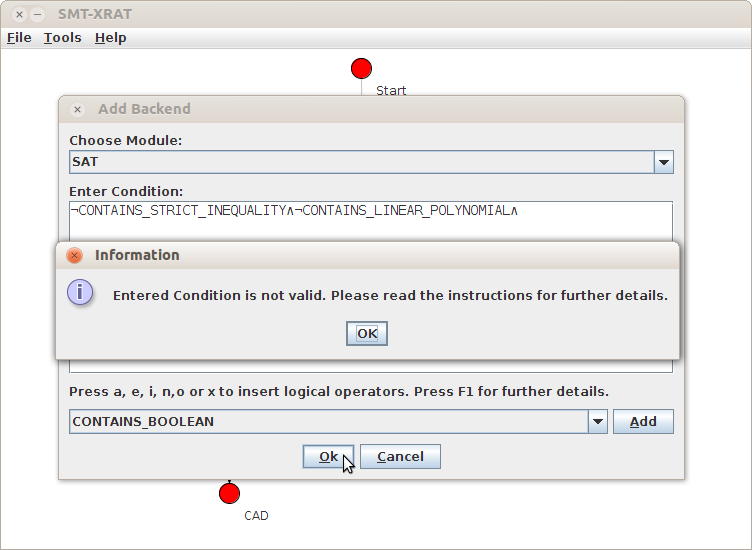
\includegraphics[width=0.9\textwidth]{graphics/smt-xrat_condition_wrong.png}
  \end{center}
  \caption{A wrong condition has been inputted by the user.}
  \label{fig:smt-xrat_condition_wrong}
\end{figure}

\subsubsection{Manipulating the strategy graph}
\label{sec:manipulating_the_strategy_graph}
Besides the capability of adding modules, the strategy graph pane gives the user
also the possibility to remove and edit them subsequently.

The deletion of a single module implicates that all of its succeeding modules in
the composition hierarchy will be removed as well. The strategy graph pane is only
allowed to contain one weakly connected graph. Furthermore, when deleting
one or implicitly more modules, the priority values of all remaining modules might
automatically be adjusted to comply the constraints of the priority values (the priority
value of an edge is always greater than the priority values of its preceding edges).
However, the logical priority order remains untouched.

When editing modules, the same dialog window is displayed as for adding modules.
The window components are already filled in with the attributes of the corresponding
module. However, priority values are not manipulated via this dialog window. As said before,
priority values are automatically assigned, when a module is created, and they are 
displayed alongside the edges. The user can manually change the priority order by 
pushing the priority value of a lower prioritized module in front of the priority
value of a higher prioritized one. The user achieves this by using the mouse pointer
to draw a dashed arrow from the edge label of that lower prioritized module to the
edge label of the higher prioritized module, as it is illustrated by Figure~\ref{fig:smt-xrat_priority_a}. Afterwards the lower prioritized module will have a higher
priority than the other one. The priority values of the modules might just be swapped.
If this is not possible, the priority values of the modules and of their preceding modules
are adjusted automatically, so that as a result, the newly prioritized module will be
ordered logically before the other one. The adaptation of the priority values is
emphasized by Figure~\ref{fig:smt-xrat_priority_b}.
\begin{figure}[ht]
  \begin{center}
    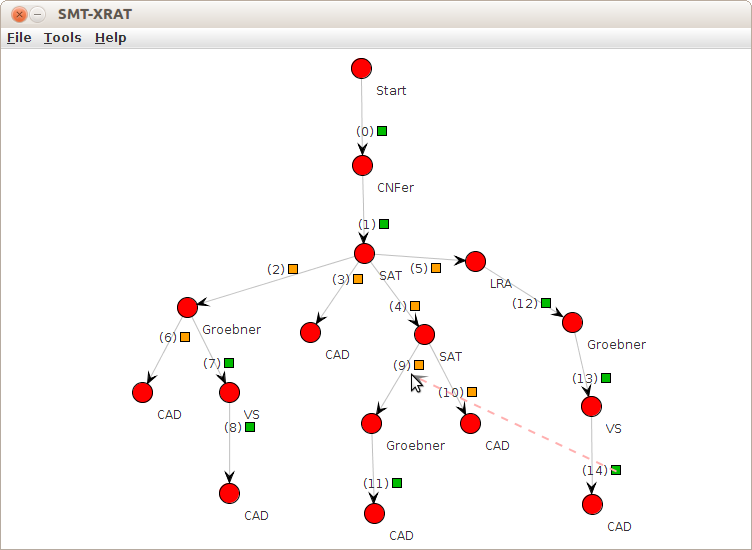
\includegraphics[width=0.9\textwidth]{graphics/smt-xrat_priority_a.png}
  \end{center}
  \caption{Priority values before changes are set.}
  \label{fig:smt-xrat_priority_a}
\end{figure}

\begin{figure}[ht]
  \begin{center}
    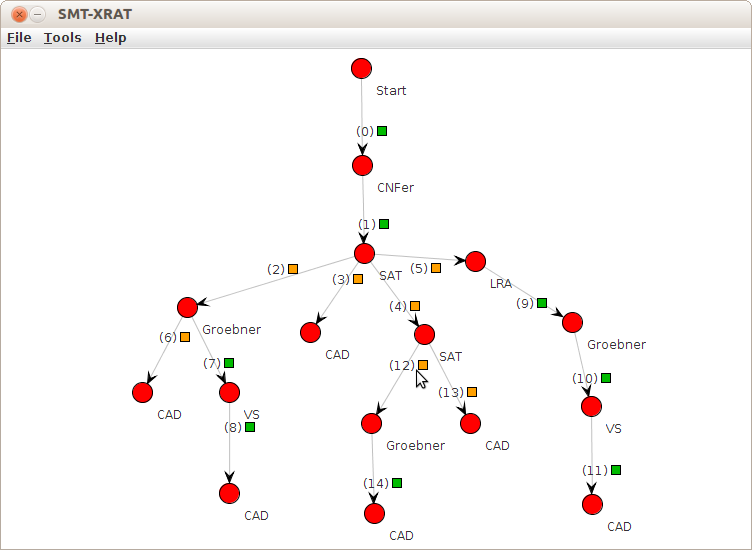
\includegraphics[width=0.9\textwidth]{graphics/smt-xrat_priority_b.png}
  \end{center}
  \caption{Intentionally changed and automatically adapted priority values.}
  \label{fig:smt-xrat_priority_b}
\end{figure}

\subsection{Further functionalities}
\label{sec:further_functionalities}
Further features of the GUI are reached through the menu bar. The most important
and also necessary functionality is the management of strategy graphs inside
the \smtrat source code, \eg the translation of a strategy in the GUI into source code
of \smtrat. To export a currently modeled strategy graph, the user simply needs 
to open the corresponding dialog window and choose a name. Figure~\ref{fig:managing_smt_solvers}
shows an example for exporting the current strategy graph and naming it 
\smtxrat. The GUI will then fulfill the translation and integration process. 
The same dialog window also lists all existing strategy graphs, which are currently 
integrated in the source code, and gives the opportunity to delete them separately.
This can be seen for the existing strategy graph \emph{NRATSolver} of the example.

The remaining features hold by the menu bar are not mandatory, but improve the creation 
process and usability. For example, the GUI allows the user to save the current strategy
graph into an XML file. This file can then be opened again for later editing or it can be
exchanged with another user. Another practical feature is the ability to save a screen shot
of the strategy graph pane into an image file. Such image files can be used to discuss
strategy graphs, when it is not desired to run the GUI.
\begin{figure}[ht]
  \begin{center}
    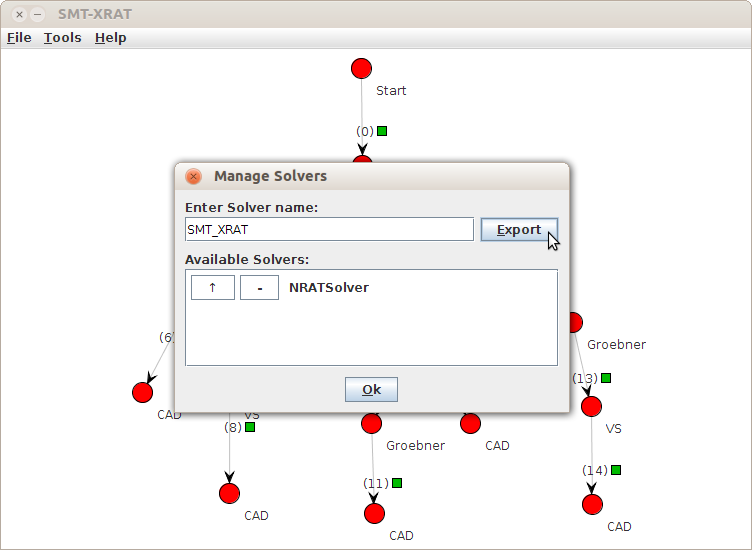
\includegraphics[width=0.9\textwidth]{graphics/smt-xrat_manage_solvers.png}
  \end{center}
  \caption{Managing SMT solvers in the SMT-RAT source code.}
  \label{fig:managing_smt_solvers}
\end{figure}


